\documentclass{article}

% Remember to also load the algostyle.sty file into your project.
\usepackage{algostyle}

% Insert new packages here.

\begin{document}
\begin{question}
In the arcade game {\em Dance Dance Revolution} (DDR), players stand on a stage and hit arrows as they scroll across the screen. More specifically, a sequence of $n$ arrows (\twemoji{left arrow}, \twemoji{up arrow}, \twemoji{right arrow}, \twemoji{down arrow}) will scroll across the screen, and as each arrow hits the top of the screen, the player must stand on the corresponding arrow on the stage.

We play a variant of DDR, aptly named {\em Don't Dance Revolution} (DDR2), where the goal is to play the game like DDR but move as little as possible. The game plays like DDR except when an arrow reaches the top of the screen and the player already has a foot on the correct arrow, then the player is awarded one lazy point. If neither foot is on the correct arrow, then the player must move {\em exactly} one foot from its current location to the correct arrow on the platform.

Unfortunately, the game is a bit unforgiving: any wrong move will cause the player to lose the game and {\em all} of their lazy points. Wrong moves include:
\begin{itemize}
    \item Failing to step on the correct arrow.
    \item Moving more than one foot at any given time.
    \item Moving either foot when the player is already stepping on the correct arrow.
\end{itemize}

You are given a sequence $A$ of $n$ arrows. Assume that your left foot starts on \twemoji{left arrow} and your right foot starts on \twemoji{right arrow}, and you have memorised the entire sequence of arrows.

For example, consider the following sequence: \twemoji{up arrow} \twemoji{up arrow} \twemoji{down arrow} \twemoji{down arrow}. We can earn up to two lazy points as follows:

\begin{center}
    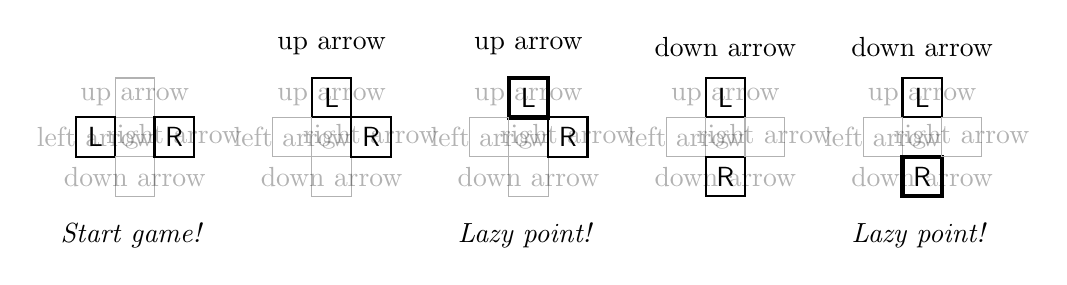
\begin{tikzpicture}
        \draw[draw = black!30] (0, 0) rectangle ++(0.5, 0.5);
        \draw[draw = black, thick] (-0.5, -0.5) rectangle ++(0.5, 0.5);
        \draw[draw = black!30] (0, -1) rectangle ++(0.5, 0.5);
        \draw[draw = black, thick] (0.5, -0.5) rectangle ++(0.5, 0.5);

        \node[opacity = 0.3] at (0.75, -0.25) {\twemoji{right arrow}};
        \node[opacity = 0.3] at (0.25, 0.25) {\twemoji{up arrow}};
        \node[opacity = 0.3] at (-0.25, -0.25) {\twemoji{left arrow}};
        \node[opacity = 0.3] at (0.25, -0.75) {\twemoji{down arrow}};
        \node[thick] at (-0.25, -0.25) {$\mathsf L$};
        \node[thick] at (0.75, -0.25) {$\mathsf R$};
        % \node at (-0.5, -0.5) [draw, minimum width = 0.5, minimum height = 0.5] {};

        \node at (0.2, -1.5) {{\em Start game!}};

        % First sequence.
        \draw[draw = black, thick] (2.5, 0) rectangle ++(0.5, 0.5);
        \draw[draw = black!30] (2, -0.5) rectangle ++(0.5, 0.5);
        \draw[draw = black!30] (2.5, -1) rectangle ++(0.5, 0.5);
        \draw[draw = black, thick] (3, -0.5) rectangle ++(0.5, 0.5);

        \node[opacity = 0.3] at (3.25, -0.25) {\twemoji{right arrow}};
        \node[opacity = 0.3] at (2.75, 0.25) {\twemoji{up arrow}};
        \node[opacity = 0.3] at (2.25, -0.25) {\twemoji{left arrow}};
        \node[opacity = 0.3] at (2.75, -0.75) {\twemoji{down arrow}};
        \node[thick] at (2.75, 0.25) {$\mathsf L$};
        \node[thick] at (3.25, -0.25) {$\mathsf R$};
        % \node at (-0.5, -0.5) [draw, minimum width = 0.5, minimum height = 0.5] {};

        \node at (2.75, 0.9) {\twemoji{up arrow}};
        % \node at (0.2, -1.5) {{\em Start game!}};

        % Second sequence.
        \draw[draw = black, ultra thick] (5, 0) rectangle ++(0.5, 0.5);
        \draw[draw = black!30] (4.5, -0.5) rectangle ++(0.5, 0.5);
        \draw[draw = black!30] (5, -1) rectangle ++(0.5, 0.5);
        \draw[draw = black, thick] (5.5, -0.5) rectangle ++(0.5, 0.5);

        \node[opacity = 0.3] at (5.75, -0.25) {\twemoji{right arrow}};
        \node[opacity = 0.3] at (5.25, 0.25) {\twemoji{up arrow}};
        \node[opacity = 0.3] at (4.75, -0.25) {\twemoji{left arrow}};
        \node[opacity = 0.3] at (5.25, -0.75) {\twemoji{down arrow}};
        \node[thick] at (5.25, 0.25) {$\mathsf L$};
        \node[thick] at (5.75, -0.25) {$\mathsf R$};
        % \node at (-0.5, -0.5) [draw, minimum width = 0.5, minimum height = 0.5] {};

        \node at (5.25, 0.9) {\twemoji{up arrow}};
        \node at (5.2, -1.5) {{\em Lazy point!}};

        % Third sequence.
        \draw[draw = black, thick] (7.5, 0) rectangle ++(0.5, 0.5);
        \draw[draw = black!30] (7, -0.5) rectangle ++(0.5, 0.5);
        \draw[draw = black, thick] (7.5, -1) rectangle ++(0.5, 0.5);
        \draw[draw = black!30] (8, -0.5) rectangle ++(0.5, 0.5);

        \node[opacity = 0.3] at (8.25, -0.25) {\twemoji{right arrow}};
        \node[opacity = 0.3] at (7.75, 0.25) {\twemoji{up arrow}};
        \node[opacity = 0.3] at (7.25, -0.25) {\twemoji{left arrow}};
        \node[opacity = 0.3] at (7.75, -0.75) {\twemoji{down arrow}};
        \node[thick] at (7.75, 0.25) {$\mathsf L$};
        \node[thick] at (7.75, -0.75) {$\mathsf R$};
        % \node at (-0.5, -0.5) [draw, minimum width = 0.5, minimum height = 0.5] {};

        \node at (7.75, 0.9) {\twemoji{down arrow}};
        % \node at (5.2, -1.5) {{\em Lazy point!}};

        % Fourth sequence.
        \draw[draw = black, thick] (10, 0) rectangle ++(0.5, 0.5);
        \draw[draw = black!30] (9.5, -0.5) rectangle ++(0.5, 0.5);
        \draw[draw = black, ultra thick] (10, -1) rectangle ++(0.5, 0.5);
        \draw[draw = black!30] (10.5, -0.5) rectangle ++(0.5, 0.5);

        \node[opacity = 0.3] at (10.75, -0.25) {\twemoji{right arrow}};
        \node[opacity = 0.3] at (10.25, 0.25) {\twemoji{up arrow}};
        \node[opacity = 0.3] at (9.75, -0.25) {\twemoji{left arrow}};
        \node[opacity = 0.3] at (10.25, -0.75) {\twemoji{down arrow}};
        \node[thick] at (10.25, 0.25) {$\mathsf L$};
        \node[thick] at (10.25, -0.75) {$\mathsf R$};
        % \node at (-0.5, -0.5) [draw, minimum width = 0.5, minimum height = 0.5] {};

        \node at (10.25, 0.9) {\twemoji{down arrow}};
        \node at (10.2, -1.5) {{\em Lazy point!}};
    \end{tikzpicture}
\end{center}

\begin{enumerate}[label = (\alph*)]
    \item Show that it is always possible to earn at least $\left\lfloor n/4 \right\rfloor$ lazy points during a round of DDR2.

    \item Describe an $O(n)$ algorithm to determine the maximum number of lazy points you can earn in a round of DDR2.

    {\bfseries Hint.} {\em We only have two feet...}
\end{enumerate}
\end{question}

\begin{solution}
\begin{enumerate}[label = (\alph*)]
    \item For any sequence of four arrows, no matter the starting position of your feet, 
    it is possibe to get at least one point.

    If any arrow appears at least twice in the sequence, then not taking the foot off the first 
    occurence of that arrow will result in scoring a lazy point when the second occurence  
    reaches the top of the screen.

    Otherwise, all arrows appear exactly once in the sequence.
    This means that at least one of the arrows in the sequence 
    will be the same as one of the arrows you are standing on initially.
    If you only move your other foot, then you will earn a lazy point when that arrow 
    reaches the top of the screen.

    Therefore within each sequence of four arrows it is always possible to earn one lazy point, 
    and so it is always possible to earn at least $\lfloor n/4\rfloor$ lazy points
    during a round.

    \pagebreak

    \item 

    \textbf{Subproblems}

    Let $S=\{\twemoji{left arrow}, \twemoji{up arrow}, \twemoji{right arrow}, \twemoji{down arrow}\}$.
    For $p_L, p_R \in S$ and $1\leq i \leq n$,
    let $P(i, p_L, p_R)$ be the problem of determining the maximum number of lazy points you can earn 
    up until the $i$-th arrow, such that $p_L$ and $p_R$ are the final positions of the left and right foot respectively.

    Let $\mathrm{opt}(i, p_L, p_R)$ be the result of $P(i, p_L, p_R)$.
    This function should return $-\infty$ if a playthrough is impossible without violating the strict rules.

    \textbf{Recurrence}

    We consider each possible positioning $(x,y)$ of both feet on the previous arrow, and choose the most optimal.
    If the previous positioning is not valid, or it is impossible to get from the previous positioning $(x,y)$ to the 
    current positioning $(p_L, p_R)$ without violating a rule, then the result of that subproblem is $-\infty$.

    $$\mathrm{opt}(i,p_L, p_R) = \begin{cases}
        -\infty &\text{if $A[i]\notin \{p_L, p_R\}$}\\
        \displaystyle\max_{\substack x, y\in S}
        \begin{cases}
            -\infty &\text{if $x\neq p_L$ and $y\neq p_R$}\\
            1 + \mathrm{opt}(i-1, x, y) &\text{if $x=p_L$ and $y=p_R$}\\
            -\infty &\text{if $A[i]\in (x, y)$}\\
            \mathrm{opt}(i-1, x, y) &\text{otherwise}\\
        \end{cases} &\text{otherwise}
        
    \end{cases}    $$

    \textbf{Base Cases}

    We can use a dummy subproblem for our base case. For all $p_L, p_R \in S$,
    $$\mathrm{opt}(0,p_L, p_R) = \begin{cases}
        0 &\text{if $p_L = \twemoji{left arrow}$ and $p_R = \twemoji{right arrow}$}\\
        -\infty&\text{otherwise}
    \end{cases}    $$

    \textbf{Order of Computation}

    Solve the subproblems in increasing order of $i$. Within the same $i$, solve in any order.

    \textbf{Overall Answer}
    
    $$\displaystyle\max_{\substack x, y\in S}\mathrm{opt}(n,x,y).$$

    \textbf{Time Complexity}

    There are $4\times 4\times n$ subproblems which is $O(n)$, each taking $O(1)$ time to solve.
    The final answer takes $O(1)$ time to extract. Thus the total time complexity is $O(n)$.


\end{enumerate}
\end{solution}
\end{document}